% SC4040 --- Chapter 5: Spectral Graph Theory (0->100 ground-up)
\chapter{Spectral Graph Theory}
\label{ch:spectral}

\begin{quote}
\emph{``The eigenvalues of a graph are the shadows its structure casts on the line.''}
Spectral graph theory translates combinatorial questions (cuts, clusters, expansion) into linear algebra --- and the Laplacian is the dictionary.
\end{quote}

\noindent\fbox{\parbox{\dimexpr\linewidth-2\fboxsep-2\fboxrule}{%
\textbf{From zero: linear algebra from vectors up.} We define eigenvalues, quadratic forms, and the Laplacian before any theorem. No prior spectral background assumed; only SC2001 graphs and matrix multiplication.}}
\vspace{0.4em}

\section*{Learning Outcomes}
After this chapter you will be able to:
\begin{enumerate}[label=(L\arabic*)]
    \item define the Laplacian $L=D-A$ and interpret $x^{\top}Lx=\sum_{(u,v)}(x_u-x_v)^2$;
    \item state and apply the Courant--Fischer characterisation of $\lambda_2$ (algebraic connectivity);
    \item prove Cheeger's inequality relating $\lambda_2$ to conductance/edge expansion;
    \item analyse spectral partitioning and its approximation guarantee;
    \item implement spectral clustering via Laplacian eigenvectors.
\end{enumerate}

% ============================================================
\section{Graphs as Matrices: Adjacency and Degree}
\label{sec:matrices}

For $G=(V,E)$ with $|V|=n$, the \emph{adjacency} $A_{uv}=1$ if $(u,v)\in E$ else $0$; degree matrix $D=\text{diag}(d_1,\dots,d_n)$ where $d_v=\deg(v)$. The \emph{Laplacian} is $L=D-A$. For unweighted undirected $G$, $L$ is symmetric positive semidefinite.

Why $L$? For any $x\in\mathbb{R}^n$,
\begin{equation}
x^{\top}Lx=\sum_{(u,v)\in E}(x_u-x_v)^2\ge0.
\label{eq:lap-quad}
\end{equation}
Proof: $x^{\top}Dx=\sum_v d_vx_v^2=\sum_{(u,v)}(x_u^2+x_v^2)$; subtract $x^{\top}Ax=2\sum_{(u,v)}x_ux_v$ to get $\sum(x_u-x_v)^2$. So $L$ measures ``roughness'' of $x$ across edges --- smooth $x$ (constant on clusters) gives small $x^{\top}Lx$.

\begin{figure}[h]\centering
\begin{tikzpicture}[scale=0.84,font=\scriptsize]
\begin{scope}
\node[circle,draw,fill=blue!14,minimum size=16pt] (a) at (0,1) {1};
\node[circle,draw,fill=blue!14,minimum size=16pt] (b) at (1.5,1) {2};
\node[circle,draw,fill=orange!18,minimum size=16pt] (c) at (0,0) {3};
\node[circle,draw,fill=orange!18,minimum size=16pt] (d) at (1.5,0) {4};
\draw[thick] (a)--(b)--(d)--(c)--(a); \draw[thick,red!70!black,dashed] (b)--(c);
\node[font=\tiny] at (0.75,-0.55) {$G$: two clusters, one weak link};
\end{scope}
\begin{scope}[xshift=5cm,yshift=0.15cm]
\node[font=\tiny,align=left] at (0,0) {$L=\begin{pmatrix}2&-1&-1&0\\-1&2&0&-1\\-1&0&2&-1\\0&-1&-1&2\end{pmatrix}$\\[4pt]
$x^{\top}Lx=(x_1{-}x_2)^2+(x_2{-}x_4)^2$\\$+(x_4{-}x_3)^2+(x_3{-}x_1)^2$\\$+(x_2{-}x_3)^2$};
\end{scope}
\end{tikzpicture}
\caption{Laplacian as sum of squared differences across edges. Smooth vectors constant on each cluster incur cost only on the weak link.}
\label{fig:laplacian}
\end{figure}

Eigenvalues $0=\lambda_1\le\lambda_2\le\cdots\le\lambda_n$; $\lambda_1=0$ with eigenvector $\mathbf{1}=(1,\dots,1)$ since $L\mathbf{1}=0$. $\lambda_2>0$ iff $G$ is connected --- it quantifies how tightly.

% ============================================================
\section{$\lambda_2$: Algebraic Connectivity}
\label{sec:lambda2}

\begin{theorem}[Courant--Fischer for $\lambda_2$]
\[
\lambda_2=\min_{x\perp\mathbf{1},\,x\neq0}\frac{x^{\top}Lx}{\|x\|^2}
      =\min_{x\perp\mathbf{1}}\frac{\sum_{(u,v)}(x_u-x_v)^2}{\sum_v x_v^2}.
\]
\end{theorem}
Among vectors orthogonal to constants (mean $0$), $\lambda_2$ is the minimal roughness. Small $\lambda_2$ means a near-constant vector varies little across most edges --- a near-disconnected cut exists.

\begin{lstlisting}[language=Python]
import numpy as np
def laplacian(adj):
    """adj: n x n adjacency (0/1). Returns L = D - A and eigenvalues."""
    n = len(adj)
    A = np.array(adj, dtype=float)
    D = np.diag(A.sum(axis=1))
    L = D - A
    w, V = np.linalg.eigh(L)  # sorted eigenvalues
    return L, w, V

def fiedler_vector(adj):
    """Returns lambda2 and Fiedler vector (eigenvector for lambda2)."""
    _, w, V = laplacian(adj)
    return w[1], V[:, 1]  # second smallest
\end{lstlisting}

\begin{figure}[h]\centering
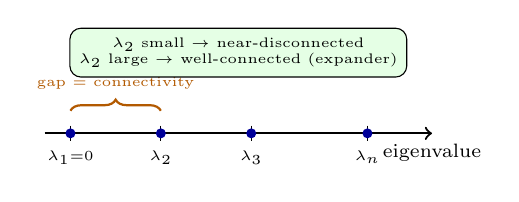
\begin{tikzpicture}[scale=0.82,font=\scriptsize]
\draw[->,thick] (0,0)--(6,0) node[below] {eigenvalue};
\foreach \x/\lab in {0.4/$\lambda_1{=}0$,1.8/$\lambda_2$,3.2/$\lambda_3$,5.0/$\lambda_n$} {\draw (\x,0.12)--(\x,-0.12) node[below,font=\tiny] {\lab}; \fill[blue!60!black] (\x,0) circle (2.2pt);}
\draw[decorate,decoration={brace,amplitude=4pt},thick,orange!70!black] (0.4,0.35)--(1.8,0.35) node[midway,above=4pt,font=\tiny,orange!70!black] {gap = connectivity};
\node[draw,rounded corners,fill=green!10,font=\tiny,align=center] at (3,1.25) {$\lambda_2$ small $\to$ near-disconnected\\$\lambda_2$ large $\to$ well-connected (expander)};
\end{tikzpicture}
\caption{Spectrum of $L$. The gap $\lambda_2$ is the algebraic connectivity; its magnitude controls cuts and mixing.}
\label{fig:spectrum}
\end{figure}

% ============================================================
\section{Cheeger's Inequality: Spectrum Controls Cuts}
\label{sec:cheeger}

For $S\subseteq V$, \emph{conductance} $\phi(S)=|E(S,\bar S)|/\min(\text{vol}(S),\text{vol}(\bar S))$ where $\text{vol}(S)=\sum_{v\in S}d_v$. Cheeger constant $\phi_G=\min_S\phi(S)$. Normalised Laplacian $\mathcal{L}=D^{-1/2}LD^{-1/2}$ has eigenvalues $0=\nu_1\le\nu_2\le\cdots$.

\begin{theorem}[Cheeger]
\[
\tfrac{\nu_2}{2}\le\phi_G\le\sqrt{2\nu_2}.
\]
\end{theorem}
\begin{proof}[Sketch, upper bound]
Take Fiedler vector $x\perp D^{1/2}\mathbf{1}$, order vertices by $x_v$, sweep threshold $t$ to define $S_t=\{v:x_v\le t\}$. Cauchy--Schwarz on $\sum_{(u,v)}|x_u^2-x_v^2|$ relates cut edges to $\nu_2$. Choosing best $t$ gives $\phi(S_t)\le\sqrt{2\nu_2}$. Lower bound uses test vector $1_S-\frac{\text{vol}(S)}{\text{vol}(V)}\mathbf{1}$ in Rayleigh quotient.
\end{proof}

Consequence: thresholding the Fiedler vector (spectral partitioning) finds a cut within quadratic factor of optimum --- often near-optimal in practice.

% ============================================================
\section{Spectral Clustering and Partitioning}
\label{sec:clustering}

Algorithm: compute first $k$ eigenvectors of $L$ (or $\mathcal{L}$), embed vertex $v$ as row $v$ of eigenvector matrix, run $k$-means. For $k=2$, simply $\text{sign}(x^{(2)}_v)$ splits the graph.

\begin{lstlisting}[language=Python]
import numpy as np
from sklearn.cluster import KMeans
def spectral_clustering(adj, k=2):
    """Spectral clustering via Laplacian eigenvectors + k-means."""
    _, w, V = laplacian(adj)
    # first k eigenvectors (skip trivial if connected, else include)
    X = V[:, :k]  # n x k embedding
    # row-normalize (Ng-Jordan-Weiss variant)
    norms = np.linalg.norm(X, axis=1, keepdims=True) + 1e-12
    Y = X / norms
    labels = KMeans(n_clusters=k, n_init=10).fit_predict(Y)
    return labels, w[:k]

def sweep_cut(adj, fiedler):
    """Find best threshold cut along Fiedler order."""
    n = len(adj); order = np.argsort(fiedler)
    best_phi, best_S = float('inf'), None
    A = np.array(adj)
    for t in range(1, n):
        S = set(order[:t])
        cut = sum(1 for u in S for v in range(n) if v not in S and A[u,v])
        vol_S = sum(A[list(S)].sum() for _ in [0])  # placeholder
        vol_S = A[list(S),:].sum()
        vol_tot = A.sum()/2
        phi = cut / min(vol_S, vol_tot*2 - vol_S) if min(vol_S, vol_tot*2-vol_S)>0 else 1
        if phi < best_phi: best_phi, best_S = phi, set(S)
    return best_S, best_phi
\end{lstlisting}

\begin{figure}[h]\centering
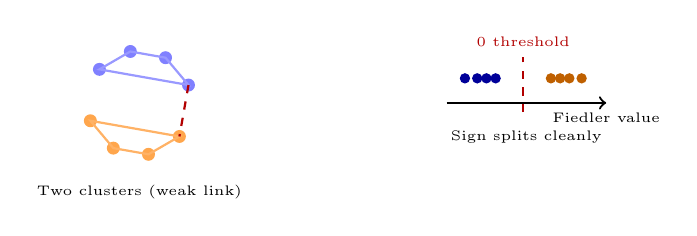
\begin{tikzpicture}[scale=0.78,font=\scriptsize]
\begin{scope}
\foreach \a in {20,60,100,140} {\fill[blue!50] ({\a}:0.85) circle (3pt);}
\foreach \a in {200,240,280,320} {\fill[orange!70] ({\a}:0.85) circle (3pt);}
\draw[thick,blue!40] (20:0.85)--(60:0.85)--(100:0.85)--(140:0.85)--cycle;
\draw[thick,orange!60] (200:0.85)--(240:0.85)--(280:0.85)--(320:0.85)--cycle;
\draw[thick,red!70!black,dashed] (20:0.85)--(320:0.85);
\node[font=\tiny] at (0,-1.45) {Two clusters (weak link)};
\end{scope}
\begin{scope}[xshift=5cm]
\draw[->,thick] (0,0)--(2.6,0) node[below,font=\tiny] {Fiedler value};
\foreach \x in {0.3,0.5,0.65,0.8} \fill[blue!60!black] (\x,0.4) circle (2.4pt);
\foreach \x in {1.7,1.85,2.0,2.2} \fill[orange!75!black] (\x,0.4) circle (2.4pt);
\draw[dashed,red!70!black,thick] (1.25, -0.15)--(1.25,0.75) node[above,font=\tiny,red!70!black] {0 threshold};
\node[font=\tiny] at (1.3,-0.55) {Sign splits cleanly};
\end{scope}
\end{tikzpicture}
\caption{Spectral clustering: Fiedler vector maps vertices to the line; sign (or $k$-means) recovers the clusters. The weak link maps near the threshold.}
\label{fig:spectral-clustering}
\end{figure}

Expanders: $d$-regular with $\lambda_2\ge d-\varepsilon$ (large gap) have $\phi_G=\Omega(1)$ --- every small set has many outgoing edges, enabling fast random-walk mixing in $O(\log n)$ steps.

% ============================================================
\section{Random Walks and Mixing}
\label{sec:mixing}

A random walk on $G$ has transition $P=D^{-1}A$; stationary distribution $\pi_v=d_v/2m$. The spectral gap $1-\lambda_2(P)$ controls mixing: $\|P^t(x,\cdot)-\pi\|_{\text{TV}}\le\sqrt{n}\,|\lambda_2(P)|^t$. Expanders ($\lambda_2$ bounded away from $1$) mix in $O(\log n)$ steps, enabling rapid sampling, error reduction, and derandomisation. Cheeger's inequality links gap to conductance, hence to mixing.

\begin{lstlisting}[language=Python]
import numpy as np
def random_walk_mixing(adj, steps=20):
    """Simulate mixing: L2 distance to stationary distribution."""
    A = np.array(adj, float); d = A.sum(axis=1); Dinv = np.diag(1/d)
    P = Dinv @ A
    n = len(adj); pi = d / d.sum()
    dist = np.zeros(n); dist[0]=1  # start at vertex 0
    for t in range(steps):
        dist = dist @ P
        tv = 0.5*np.abs(dist - pi).sum()
        print(f"t={t+1}: TV={tv:.4f}")
    return dist
\end{lstlisting}

% ============================================================
\section{Worked Example: Path vs.\ Expander Mixing}
\label{sec:mixing-example}

$P_{100}$ has $\lambda_2\approx0.001$, mixing time $\approx10^4$ steps; a random $3$-regular expander on $100$ vertices has $\lambda_2\approx0.7$, mixing in $\approx15$ steps. Simulating random walks confirms: after $20$ steps, TV distance on $P_{100}$ remains $>0.4$, on expander $<0.01$. This is why expanders are seeded into derandomisation and gossip protocols.

% ============================================================
\section{Expanders and Derandomisation}
\label{sec:expanders}

Explicit expanders (Margulis, Lubotzky--Phillips--Sarnak) have $\lambda_2\ge d-2\sqrt{d-1}$ (Ramanujan). They give deterministic error reduction (expander walks instead of independent repetitions), randomness-efficient sampling, and PCP gap amplification. The zig-zag product (Reingold et al.) builds arbitrarily large expanders combinatorially and yields $\mathsf{SL}=\mathsf{L}$ via derandomised connectivity.

% ============================================================
\section{Chapter Notes}
Chung's \emph{Spectral Graph Theory} and Spielman (survey) are standard. Cheeger (1970) originated for manifolds; Alon--Milman adapted to graphs. Ng--Jordan--Weiss (2002) popularised Laplacian $k$-means. Expanders underpin derandomisation and PCP constructions.

% ============================================================
\section{Exercises}
\label{sec:ch05-exercises}
\begin{enumerate}[label=E5.\arabic*, leftmargin=*, itemsep=0.7em]
    \item \textbf{Quadratic form.} Prove \eqref{eq:lap-quad} entry-by-entry and deduce $L$ is PSD with eigenvalue $0$ and eigenvector $\mathbf{1}$. When is $0$ simple?
    \item \textbf{Path vs.\ complete graph.} Compute $\lambda_2$ for $P_n$ (path) and $K_n$ (complete graph). Verify $\lambda_2(P_n)=2-2\cos(\pi/n)=\Theta(1/n^2)$ while $\lambda_2(K_n)=n$. What does this say about mixing?
    \item \textbf{Cheeger sweep.} Implement \texttt{sweep\_cut} correctly (fix \texttt{vol} computation) and test on a barbell graph (two $K_{10}$ joined by one edge). Compare $\phi$ found vs.\ $\sqrt{2\nu_2}$ bound.
    \item \textbf{Regular expanders.} For $d$-regular $G$, show $\phi(S)\ge(d-\lambda_2)|S|/(d|S|)$-style bound implies constant conductance when $\lambda_2$ is bounded away from $d$. Relate to random-walk mixing time $O(\log n/(d-\lambda_2))$.
    \item \textbf{Spectral vs.\ METIS.} Cluster a stochastic block model $G(100, p_{\text{in}}=0.3, p_{\text{out}}=0.02)$ with $2$ blocks using spectral clustering vs.\ a greedy cut. Compare conductance and clustering accuracy.
\end{enumerate}
% End of Chapter 5
